\section{Experiments}

\subsection{Reproducing the results of \textcite{frenayParameterinsensitiveKernelExtreme2011}}
\label{sec:reproducing-frenay}

% \begin{figure}[H]
% 	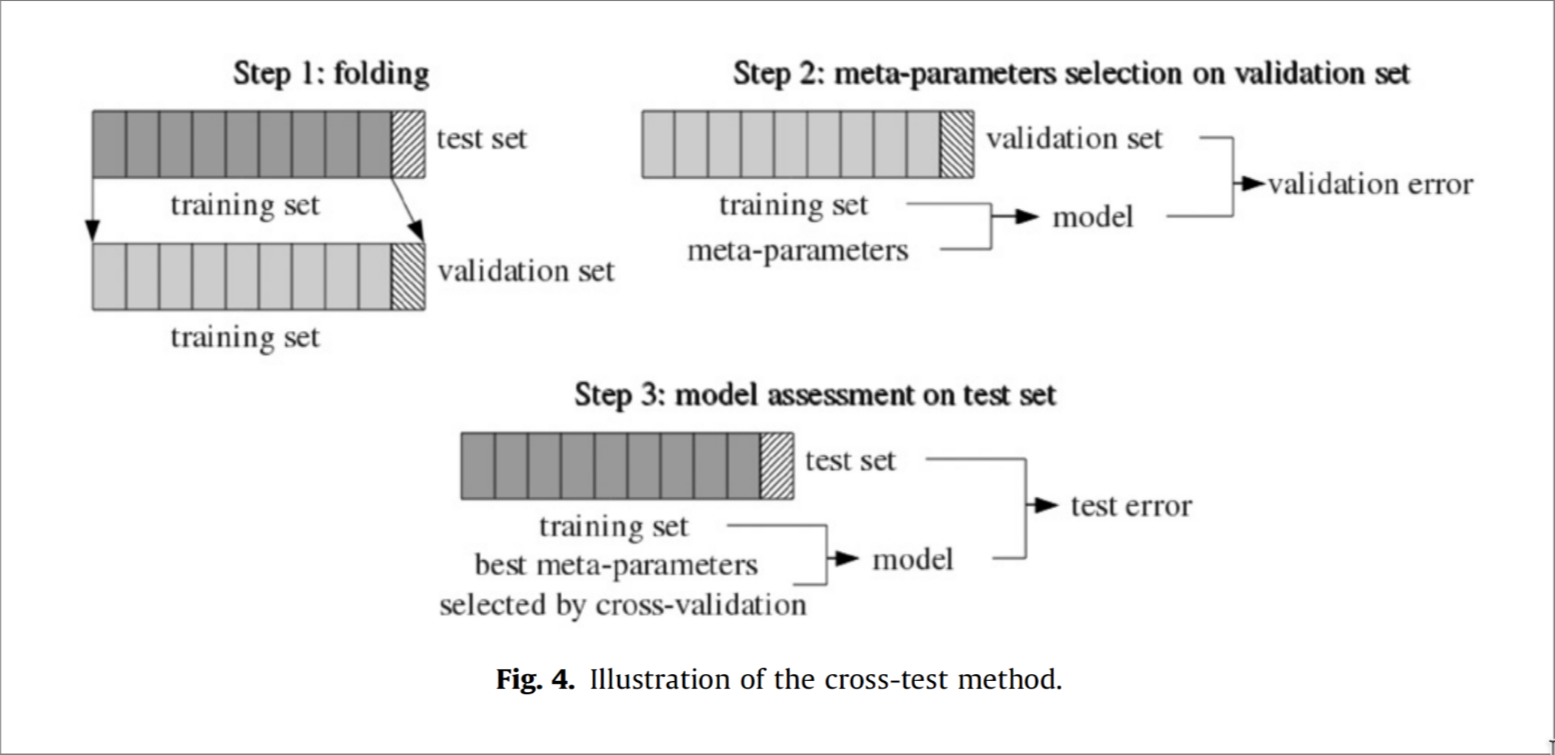
\includegraphics{frenay-cross-test}
% 	\caption{Illustration of the cross-test method from \cite{frenayParameterinsensitiveKernelExtreme2011}}
% 	\label{fig:frenay-cross-test}
% \end{figure}

In the paper, \textcite{frenayParameterinsensitiveKernelExtreme2011} use a double cross-test resampling
method which is illustrated in \cref{fig:frenay-cross-test}. First, they perform a 10-fold cross validation,
where the 9 folds of the training set are then used on a second 10-fold cross validation to determine the
best hyperparameters. This means that there are 100 training processes in total.

\begin{figure}[H]
    \begin{tikzpicture}[
		scale=0.66,
		every node/.style={font=\footnotesize},
	]
	% Draw main rectangle
	\def\nfolds{10}
	\pgfmathsetmacro{\trainfolds}{\nfolds-1}
	\pgfmathsetmacro{\splits}{\nfolds-2}
	\def\heightmult{0.5}

	\newcommand{\fold}[5]{%
		\draw[#2] #1 rectangle ($#1+(\heightmult*\trainfolds,1)$);
		% fill with pattern
		\filldraw[#3] ($#1+(\heightmult*\trainfolds,0)$) rectangle ($#1+(\heightmult*\nfolds,1)$);

		\draw ($#1+(\heightmult*\trainfolds/2,0)$) node[below,name=below-#5] {training set};
		\draw ($#1+(\heightmult*\nfolds,0.5)$) node[right,name=right-#5] {#4 set};

		% Draw vertical dashed lines for fold divisions
		\foreach \x in {1,...,\splits}{
				\draw ($#1+(\heightmult*\x,0)$) -- ($#1+({\heightmult*\x},1)$);
			}
	}

	\def\coltest{wong_blue}
	\def\colvali{wong_orange}

	\fill[shading=axis,top color=\coltest!40,bottom color=\colvali!40] (0,0) -- (\heightmult*\trainfolds,0) -- (\heightmult*\nfolds,-1) -- (0,-1) -- cycle;

	\fold{(0,0)}{fill=\coltest}{pattern=north east lines, pattern color=\coltest}{test}{test1}
	\fold{(0,-2)}{fill=\colvali}{pattern=north west lines,pattern color=\colvali}{validation}{val1}

	\draw[->] (0,0) -- (0,-1);
	\draw[->] (\heightmult*\trainfolds,0) -- (\heightmult*\nfolds,-1);

	% title above bounding box
	% \draw (current bounding box.north) node[above] {\textbf{Step 1: folding}};

	\fold{(9,0)}{fill=\colvali}{pattern=north west lines,pattern color=\colvali}{validation}{val2}

	\draw (right-val1.east -| below-val2.south) node[name=meta-parameters] {meta-parameters};
	\coordinate (a) at ($(meta-parameters)!.5!(below-val2)$);
	\node[name=model] at (a -| right-val2) {model};

	\coordinate (vm) at ($(model)!.5!(right-val2)$);
	\node[name=valerr] at ($(vm)+(5,0)$) {validation error};

	\coordinate (mm) at ($(meta-parameters.east |- model.west)!0.5!(model.west)$);
	\draw (below-val2.east) -| (mm);
	\draw (meta-parameters.east) -| (mm);
	\draw[->] (mm) -- (model);

	\coordinate (vvm) at ($(right-val2.east |- valerr.west)!0.5!(valerr.west)$);
	\draw (right-val2.east) -| (vvm);
	\draw (model.east) -| (vvm);
	\draw[->] (vvm) -- (valerr);

	% step 3

	\coordinate (step3) at (5,-5);
	\fold{(step3)}{fill=\coltest}{pattern=north east lines,pattern color=\coltest}{test}{test3}

	\draw ($(below-test3.south)+(0,-1)$) node[name=best-meta-parameters,text width=3cm,align=center]
	{best meta-parameters selected by cross-validation};

	\coordinate (b) at ($(best-meta-parameters)!.5!(below-test3)$);
	\node[name=model3] at ($(b -| right-test3)+(1,0)$) {model};

	\coordinate (vm3) at ($(model3)!.5!(right-test3)$);
	\node[name=testerr] at ($(vm3)+(5,0)$) {test error};

	\coordinate (mm3) at ($(best-meta-parameters.east |- model3.west)!0.5!(model3.west)$);
	\draw (below-test3.east) -| (mm3);
	\draw (best-meta-parameters.east) -| (mm3);
	\draw[->] (mm3) -- (model3);

	\coordinate (vvm3) at ($(right-test3.east |- testerr.west)!0.5!(testerr.west)$);
	\draw (right-test3.east) -| (vvm3);
	\draw (model3.east) -| (vvm3);
	\draw[->] (vvm3) -- (testerr);

	\coordinate (shift) at (0,1.5);
	\draw ($(0,0)+(shift)$) node[right] {\textbf{Step 1: folding}};
	\draw ($(9,0)+(shift)$) node[right] {\textbf{Step 2: meta-parameters selection on validation set}};
	\draw ($(step3)+(shift)$) node[right] {\textbf{Step 3: model assessment on test set}};

	% \draw ($(9,0)!0.5!(valerr.east) + (0,1.1)$) node[above] {\textbf{Step 2: meta-parameters selection on validation set}};

	% \draw ($(step3)!0.5!(step3 -| testerr.east) + (0,1)$) node[above] {\textbf{Step 3: model assessment on test set}};

\end{tikzpicture}

	\caption{Illustration of the cross-test method from \cite{frenayParameterinsensitiveKernelExtreme2011}}
	\label{fig:frenay-cross-test}
\end{figure}

\subsection{Comparing the performance of the kernels with different datasets}

\begin{figure}
    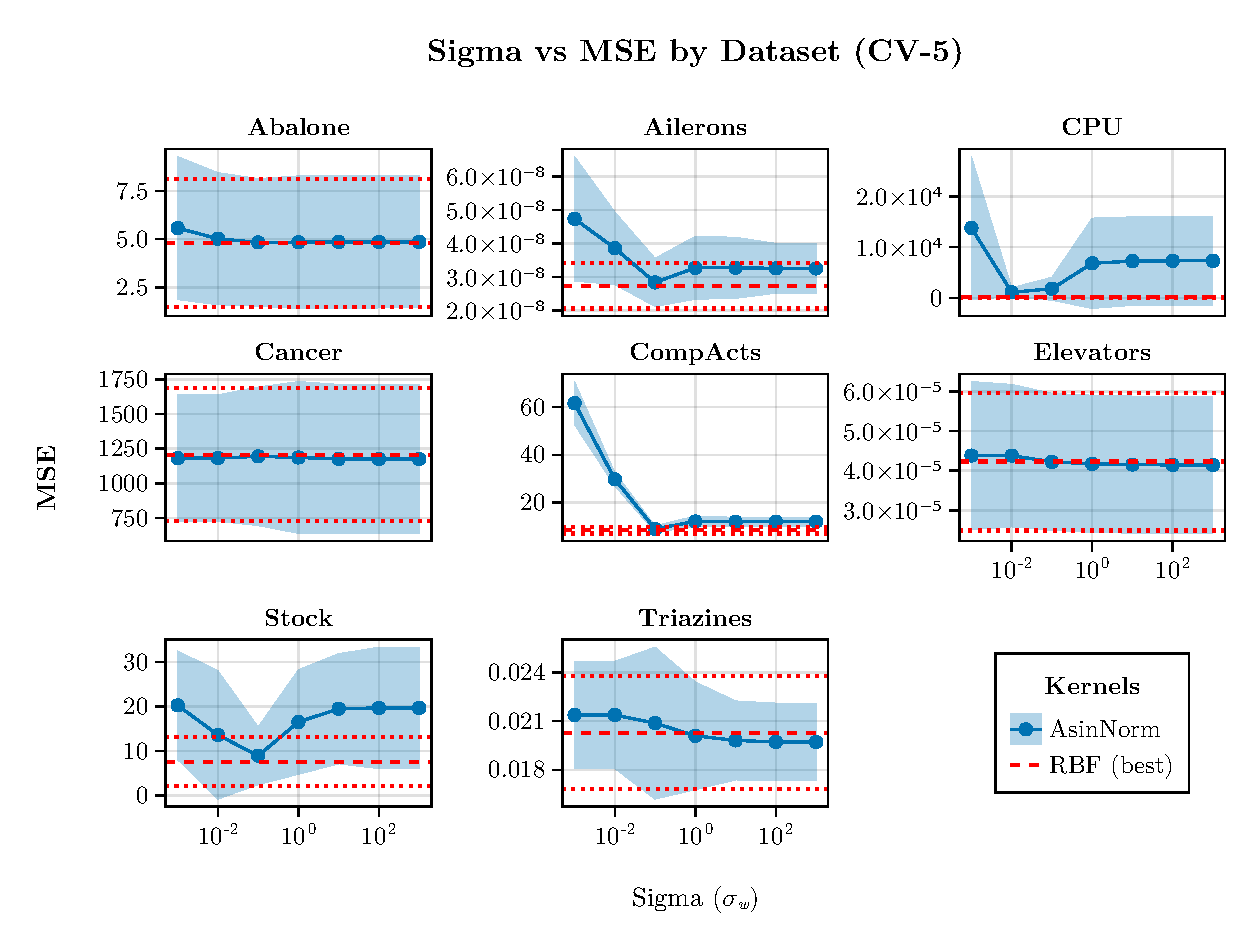
\includegraphics{../plots/MSE_frenay}
    \caption{MSE results on datasets from \cite{frenayParameterinsensitiveKernelExtreme2011}}
\end{figure}

\subsubsection{Resampling}

Instead of using the double cross-test resampling used in \cref{sec:reproducing-frenay},
we opted to use a 5-2 cross-validation resampling method as described by \textcite{dietterichApproximateStatisticalTests1998}.

The 5-2 cross-validation
consists of doing a 50-50 split of the dataset into two sets. First, we train on the first set and test on the second set
and then we train on the second set and test on the first set. The process is repeated 5 times, each time
with a different random split. We choose this method since it is faster than the double cross-test method
requiring only 10 training processes instead of 100.

% TODO: Add figure of the 5-2 cross-validation

\subsubsection{Normalization}

In order to be able to compare the results between different datasets, an effort
was made to normalize the data and hyperparameters. To that end, the
following measures were implemented:

\begin{enumerate}
    \item Variables (including target) are standardized
    \item We use normalized root-mean-square error as our performance
        measure.
    \item The kernel itself is normalized.
    \item The hyperparameter $\sigma_w$ is divided by the number of samples in
        the training data of each dataset.
\end{enumerate}



% NOTE: this is without scaling sigma
\begin{figure}
    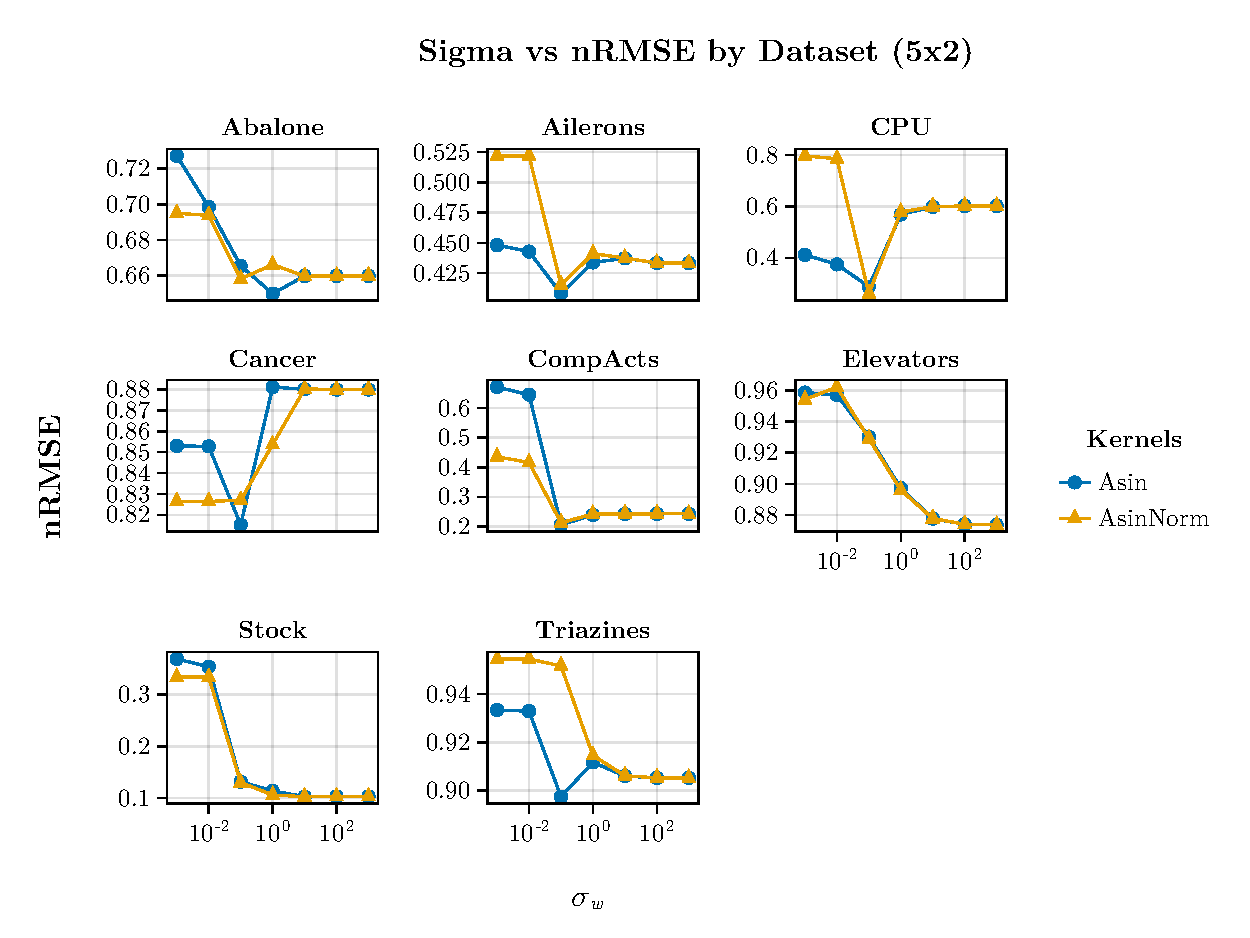
\includegraphics{../plots/nRMSE_frenay}
    \caption{nRMSE results on datasets from \cite{frenayParameterinsensitiveKernelExtreme2011}}
\end{figure}

% WARN: these don't have all values of epsilon in our grid
\begin{figure}
    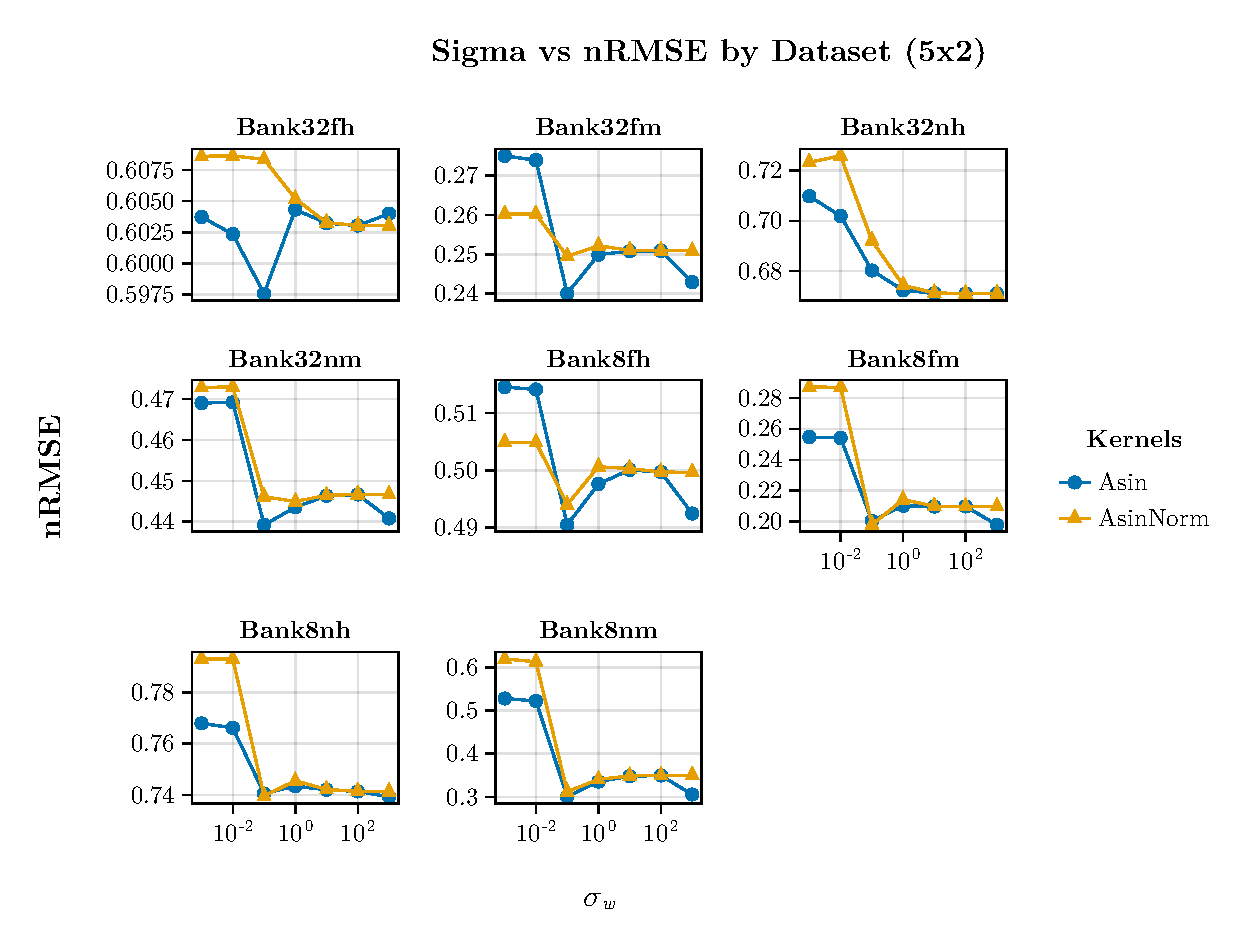
\includegraphics{../plots/nRMSE_bank}
    \caption{nRMSE results on Delve Bank dataset}
\end{figure}

% WARN: these don't have all values of epsilon in our grid
\begin{figure}
    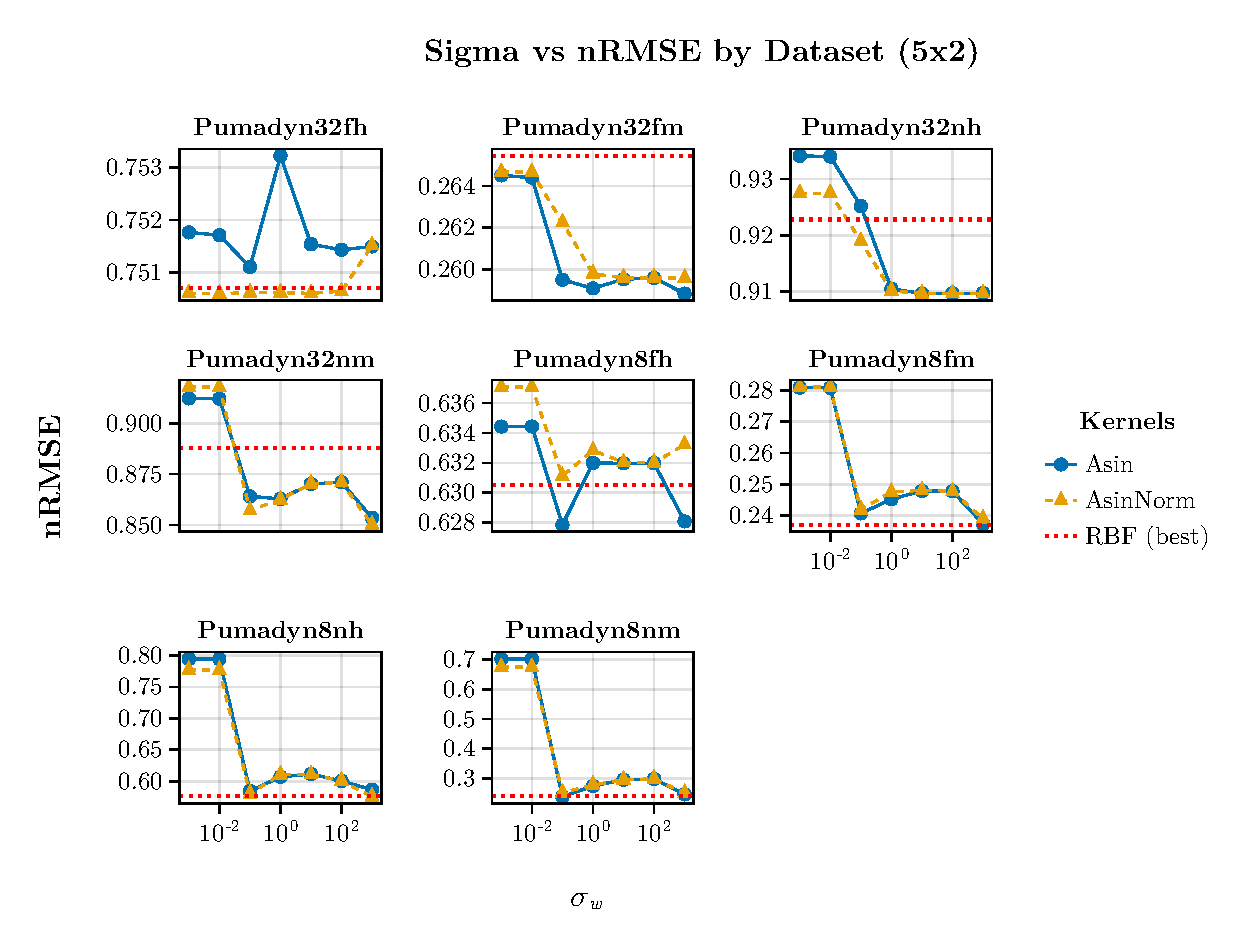
\includegraphics{../plots/nRMSE_pumadyn}
    \caption{nRMSE results on Delve PumaDyn dataset}
\end{figure}
